%%%%%%%%%%%%%%%%%%%%%%%%%%%%%%%%%%%%%%%%%%%%%%%%%%%%%%%%%%%%%%%%%%%%%%%%%
%
% Purpose: Appendices for JSC Engineering Orbital Dynamics (JEOD)
%
%
%
% 
%%%%%%%%%%%%%%%%%%%%%%%%%%%%%%%%%%%%%%%%%%%%%%%%%%%%%%%%%%%%%%%%%%%%%%%%%

\chapter{Test States and Simulation Tests}\label{ap:tdata}
\begin{enumerate}
\item Total State for the Clementine vehicle.
\item Total State for the Rosetta vehicle.
\item Total State for Phobos
\item Total State for the Dawn vehicle.
\end{enumerate}

State information for the following vehicles are only available in NASA internal release of JEOD
\begin{itemize}
\item Total State for the CHAMP vehicle
\item Total State for the ISS vehicle
\item Total State for the Envisat vehicle
\item Total State for the Lageos vehicle
\item Total State for the TDRS vehicle
\item Total State for the GRACE A vehicle.
\item Total State for the GRACE B vehicle.
\end{itemize}

Location of test simulations directory verif SIM\_Integrated test runs,
where (5)-(11) are only available in the NASA internal release:
\begin{verbatim}
(1)  /verif/Integrated_Validation/SIM_Earth_Moon/SET_test/SET_test/RUN_clem
(2)  /verif/Integrated_Validation/SIM_Earth_Moon/SET_test/RUN_rosetta
(3)  /verif/Integrated_Validation/SIM_Mars/SET_test/RUN_phobos
(4)  /verif/Integrated_Validation/SIM_Mars/SET_test/RUN_dawn
(5)  /verif/Integrated_Validation/SIM_Earth_Moon/SET_test/SET_test/RUN_champ
(6)  /verif/Integrated_Validation/SIM_Earth_Moon/SET_test/SET_test/RUN_iss
(7)  /verif/Integrated_Validation/SIM_Earth_Moon/SET_test/SET_test/RUN_envisat
(8)  /verif/Integrated_Validation/SIM_Earth_Moon/SET_test/SET_test/RUN_lageos
(9)  /verif/Integrated_Validation/SIM_Earth_Moon/SET_test/SET_test/RUN_tdrs
(10) /verif/Integrated_Validation/SIM_Grace/SET_test/RUN_gracea
(11) /verif/Integrated_Validation/SIM_Grace/SET_test/RUN_graceb
\end{verbatim}


This appendix provides initial state information used in the various \JEOD\ integrated
test cases. For this set of tests, there are eleven initial orbital states with four available
for public release and additional of seven available only for the internal release version:
\newpage
\section {Test 1: Champ LEO State and Environment (Internal-Only)}\label{tbl:champic}

\section {Test 2: ISS LEO State and Environment (Internal-Only)}\label{tbl:issic}

\section {Test 3: ENVISAT HEO1 State and Environment (Internal-Only)}\label{tbl:eviic}

\section {Test 4: Lageos HEO2 State and Environment (Internal-Only)}\label{tbl:lagic}

\section {Test 5: TDRS GEO State and Environment (Internal-Only)}\label{tbl:tdrsic}

\newpage
\section {Test 6: Clementine Lunar Orbit State}\label{tbl:clemic}
\begin{table}[htb]
\begin{center}
\caption{Clementine State and Environment-Lunar Orbit} \vspace{5mm}
\begin{tabular}{|l|c|l|l|}
\hline
Epoch Data    & Units     & Value   & Description:     \\ \hline \hline
Year          & $y$       & 1994        &     Year             \\ \hline
Month         & $m$       &  03       &     Month              \\ \hline
Day           & $d$       &  1           &     Day              \\ \hline
Hour          & $h$       & 0           &     Hour               \\ \hline
Min           & $n$       & 0            &     Minute               \\ \hline
Second        & $s$       & 0.0         &     Second               \\ \hline
DUT1          & $s$       &  n/a   & UT1 - UTC        \\ \hline
Delta AT      & $s$       &  n/a       & IERS Leap Second \\ \hline \hline
$x_p$         & $as$      &  n/a2   &  X Polar Offset   \\ \hline
$y_p$         & $as$      &  n/a  &  Y Polar Offset    \\ \hline \hline
State Vector      &           &     &      \\ \hline \hline
$x_{J2000}$       & $km$      &1296.94401*    &  X Position J2000       \\ \hline
$y_{J2000}$       & $km$      & -1060.82445*   &  Y Position J2000        \\ \hline
$z_{J2000}$       & $km$      & 2522.289146*   &  Z Position J2000       \\ \hline
$\dot x_{J2000}$  &$km/s$       &-.930578    &  X Component Velocity J2000   \\ \hline
$\dot y_{J2000}$  &$km/s$       &-.439312   &  Y Component Velocity J2000    \\ \hline
$\dot z_{J2000}$  &$km/s$       & .862075  &  Z Component Velocity J2000      \\ \hline \hline
Atmosphere data   &                   &          &      \\ \hline \hline
$F_{10.7}$        & $W/{H_z}{m^2}$    & n/a    & UV Correlated Solar radio noise flux             \\ \hline
$F_{10.7B}$       & $W/{H_z}{m^2}$    &  n/a              &  90 day average UV Correlated Solar radio noise flux  \\ \hline
$a_p$             &  NA               &  n/a             &  Geomagnetic Activity Index                \\ \hline \hline
Aerodynamic data  &           &                       &      \\ \hline \hline
$C_d$             &None       &     n/a                  & Coefficient of drag \\ \hline
BC                &$kg/m^2$   &     n/a                 & Ballistic Coefficient \\ \hline
Mass              &kg         &     424.0                  & Vehicle Mass           \\ \hline
Area              &$m^2$      &    2.1432                  & Vehicle Reference Area  \\ \hline
Cr                &$None$      &    1.23                  & Vehicle Coefficient of Reflection   \\ \hline
\end{tabular}
\end{center}
\end{table}
Radial error  $ \pm $ 1.5 meters , in-track  $ \pm $ 30 meters and  $ \pm $ 10 meters cross-track, \cite{AK} .


\newpage
\section {Test 7: GRACE Orbit State (Internal-Only)}\label{tbl:gracea}

\section {Test 8: GRACE Orbit State (Internal-Only)}\label{tbl:graceb}

\newpage
\section {Test 9: Rosetta Orbit State}\label{tbl:rosetta}
\begin{table}[htb]
\begin{center}
\caption{Rosetta State and Environment} \vspace{5mm}
\scalebox{0.8}{
\begin{tabular}{|l|c|l|l|}
\hline
Epoch Data         & Units     & Value   & Description:     \\ \hline \hline
Year          & $y$       & 2009              &    Year             \\ \hline
Month         & $m$       & 11             &     Month              \\ \hline
Day           & $d$       & 13             &     Day              \\ \hline
Hour          & $h$       & 05           &     Hour               \\ \hline
Min           & $n$       & 0            &     Minute               \\ \hline
Second        & $s$       & 0.0          &     Second               \\ \hline
DUT1             & $s$ auto select      &           & UT1 - UTC        \\ \hline
Delta AT         & $s$ auto select      &           & IERS Leap Second \\ \hline \hline
$x_p$            & $as$ auto select      &           &  X Polar Offset   \\ \hline
$y_p$            & $as$ auto select     &           &  Y Polar Offset    \\ \hline \hline
State Vector         &             &          &      \\ \hline \hline
$x_{J2000}$       & $km$       &   87396.6219145        $ \pm $ 2 m*  & X Position J2000       \\ \hline
$y_{J2000}$       & $km$       &   23042.6606938             $ \pm $ 2 m*   &  Y Position J2000        \\ \hline
$z_{J2000}$       & $km$       &   -48761.8708343      $ \pm $   2 m*       & Z Position J2000   \\ \hline
$\dot x_{J2000}$  &$km/s$      &    -7.8839651            $ \pm $ .1 mm/s*    & X Component Velocity J2000    \\ \hline
$\dot y_{J2000}$  &$km/s$       &    -3.2492092    $ \pm $ .1 mm/s*    & Y Component Velocity J2000    \\ \hline
$\dot z_{J2000}$  &$km/s$       &    4.7952127   $ \pm $ .1 mm/s*     & Z Component Velocity J2000      \\ \hline \hline
Atmosphere data   &            &          &      \\ \hline \hline
$F_{10.7}$        & $W/{H_z}{m^2}$    &   N/A    & UV Correlated Solar radio noise flux             \\ \hline
$F_{10.7B}$       & $W/{H_z}{m^2}$    &   N/A    &  90 day average UV Correlated Solar radio noise flux  \\ \hline
$a_p$            &  NA                &   N/A    &  Geomagnetic Activity Index                \\ \hline \hline
Aerodynamic data         &      &      &      \\ \hline \hline
$C_d$                    &None       &  N/A         & Coefficient of drag \\ \hline
BC                       &$kg/m^2$   &  N/A          & Ballistic Coefficient \\ \hline
Mass                     &kg         &  3000.0            & Vehicle Mass           \\ \hline
Area                     &$m^2$      &  N/A             & Vehicle Reference Area  \\ \hline
\end{tabular}}
\end{center}
\end{table}
*Error analysis \cite{JPL}
\clearpage


\newpage
\section {Test 10: Phobos Orbit State}\label{tbl:phobos}
\begin{table}[htb]
\begin{center}
\caption{Phobos State and Environment} \vspace{5mm}
\scalebox{0.8}{
\begin{tabular}{|l|c|l|l|}
\hline
Epoch Data         & Units     & Value   & Description:     \\ \hline \hline
Year          & $y$       & 2010             &    Year             \\ \hline
Month         & $m$       & 09             &     Month              \\ \hline
Day           & $d$       & 10             &     Day              \\ \hline
Hour          & $h$       & 0            &     Hour               \\ \hline
Min           & $n$       & 0            &     Minute               \\ \hline
Second        & $s$       & 0.0          &     Second               \\ \hline
DUT1             & $s$ auto select      &           & UT1 - UTC        \\ \hline
Delta AT         & $s$ auto select      &           & IERS Leap Second \\ \hline \hline
$x_p$            & $as$ auto select      &           &  X Polar Offset   \\ \hline
$y_p$            & $as$ auto select     &           &  Y Polar Offset    \\ \hline \hline
State Vector         &             &          &      \\ \hline \hline
$x_{J2000}$       & $km$       &      8240.7901108     $ \pm $ 2 m*  & X Position J2000       \\ \hline
$y_{J2000}$       & $km$       &      605.0716371           $ \pm $ 2 m*   &  Y Position J2000        \\ \hline
$z_{J2000}$       & $km$       &       -4152.5375845 $ \pm $   2 m*       & Z Position J2000   \\ \hline
$\dot x_{J2000}$  &$km/s$      &      0.3077392         $ \pm $ .1 mm/s*    & X Component Velocity J2000    \\ \hline
$\dot y_{J2000}$  &$km/s$       &       1.9627295 $ \pm $ .1 mm/s*    & Y Component Velocity J2000    \\ \hline
$\dot z_{J2000}$  &$km/s$       &      0.8655744 $ \pm $ .1 mm/s*     & Z Component Velocity J2000      \\ \hline \hline
Atmosphere data   &            &          &      \\ \hline \hline
$F_{10.7}$        & $W/{H_z}{m^2}$    &   N/A    & UV Correlated Solar radio noise flux             \\ \hline
$F_{10.7B}$       & $W/{H_z}{m^2}$    &   N/A    &  90 day average UV Correlated Solar radio noise flux  \\ \hline
$a_p$            &  NA                &   N/A    &  Geomagnetic Activity Index                \\ \hline \hline
Aerodynamic data         &      &      &      \\ \hline \hline
$C_d$                    &None       &  N/A         & Coefficient of drag \\ \hline
BC                       &$kg/m^2$   &  N/A          & Ballistic Coefficient \\ \hline
Mass                     &kg         &  1.08e+16            & Vehicle Mass           \\ \hline
Area                     &$m^2$      &  N/A             & Vehicle Reference Area  \\ \hline
\end{tabular}}
\end{center}
\end{table}
*Error analysis \cite{JPL}
\clearpage


\newpage
\section {Test 11: Dawn Orbit State}\label{tbl:dawn}
\begin{table}[htb]
\begin{center}
\caption{Dawn State and Environment} \vspace{5mm}
\scalebox{0.8}{
\begin{tabular}{|l|c|l|l|}
\hline
Epoch Data         & Units     & Value   & Description:     \\ \hline \hline
Year          & $y$       & 2009             &    Year             \\ \hline
Month         & $m$       & 02             &     Month              \\ \hline
Day           & $d$       & 17             &     Day              \\ \hline
Hour          & $h$       & 23            &     Hour               \\ \hline
Min           & $n$       & 0            &     Minute               \\ \hline
Second        & $s$       & 0.0          &     Second               \\ \hline
DUT1             & $s$ auto select      &           & UT1 - UTC        \\ \hline
Delta AT         & $s$ auto select      &           & IERS Leap Second \\ \hline \hline
$x_p$            & $as$ auto select      &           &  X Polar Offset   \\ \hline
$y_p$            & $as$ auto select     &           &  Y Polar Offset    \\ \hline \hline
State Vector         &             &          &      \\ \hline \hline
$x_{J2000}$       & $km$       &      11563.3556802     $ \pm $ 2 m*  & X Position J2000       \\ \hline
$y_{J2000}$       & $km$       &      -14356.6688977           $ \pm $ 2 m*   &  Y Position J2000        \\ \hline
$z_{J2000}$       & $km$       &       6293.7046169  $ \pm $   2 m*       & Z Position J2000   \\ \hline
$\dot x_{J2000}$  &$km/s$      &       -2.2731078         $ \pm $ .1 mm/s*    & X Component Velocity J2000    \\ \hline
$\dot y_{J2000}$  &$km/s$       &       2.3801324 $ \pm $ .1 mm/s*    & Y Component Velocity J2000    \\ \hline
$\dot z_{J2000}$  &$km/s$       &      -.0229110 $ \pm $ .1 mm/s*     & Z Component Velocity J2000      \\ \hline \hline
Atmosphere data   &            &          &      \\ \hline \hline
$F_{10.7}$        & $W/{H_z}{m^2}$    &   N/A    & UV Correlated Solar radio noise flux             \\ \hline
$F_{10.7B}$       & $W/{H_z}{m^2}$    &   N/A    &  90 day average UV Correlated Solar radio noise flux  \\ \hline
$a_p$            &  NA                &   N/A    &  Geomagnetic Activity Index                \\ \hline \hline
Aerodynamic data         &      &      &      \\ \hline \hline
$C_d$                    &None       &  N/A         & Coefficient of drag \\ \hline
BC                       &$kg/m^2$   &  N/A          & Ballistic Coefficient \\ \hline
Mass                     &kg         &  1250.0            & Vehicle Mass           \\ \hline
Area                     &$m^2$      &  N/A             & Vehicle Reference Area  \\ \hline
\end{tabular}}
\end{center}
\end{table}
*Error analysis \cite{JPL}
\clearpage



\chapter{Assumptions and Limitations on Earth Orientation}\label{ap:eartho}
The use of GGM02C has important implications due to requirements contained in the GRACE geopotential campaign \cite{grace}. A non-spherical gravity field was fit using a model of the Earth's orientation that differs from the one in JEOD. The difference as of the present time is quite small. JEOD uses an Earth orientation known as the IAU-76/FK5 \cite{Bond1} and the Explanatory Supplement to the Astronomical Almanac \cite{ES1}, which conformed to an older Goddard gravity model used in Trick Dynamics in the 1990's. However in 2003 the International Earth Rotational Service (IERS) and the Jet Propulsion Laboratory adopted a system under the name J2000. The Earth orientation model simplifies polar motion and introduces a new formulation for the construction of a new RNP \cite{IERS2003}. Vallado \cite{VMcC} notes that as time goes by IAU-76/FK and J2000 models will diverge. This has been noted as a JEOD issue and will be addressed in later releases. The J2000 coordinate system is defined by( see reference \cite{IERS2003}):
\begin{enumerate}
\item Coordinate Frame: Non-Rotating Inertial,
\item Z-axis: Defined as the pole vector of the Earth Mean Equator of J2000 (where J2000 = Julian date 2451545.0 TDB (Barycentric Dynamical Time)),
\item X-axis: Defined as the cross product of the Z-axis (as defined above) and the Earth mean orbit pole of J2000 (i.e. the ecliptic pole of J2000). The X-axis of this coordinate frame is the Earth vernal equinox of J2000,
\item Y-axis: Completes a standard, right-handed coordinate frame.
\end{enumerate}
For futher information on coordinate systems see \COORDLINK

\chapter{Assumptions about Lunar Orientation}\label{ap:moono}
The Lunar orientation is extracted from the JPL Development  Ephemeris by extraction from fitted data. It should be noted that the specified non-spherical Lunar gravity model does not have an analytic RNP model similar to the Earth. The lunar libration (lunar orientation) data are present on the JPL Development  Ephemeris file, and this software uses this libration data to determine the directions of the Moon's pole and prime meridian. Further information from JPL is linked to this document see the JPL Lunar Constants document \LUNARLINK .


\chapter{Definition of RSW System} \label{ap:rsw}
The radial, in-track and cross-track coordinate system is defined by Vallado \cite{VMcC}: (The term RSW is somewhat arbitrary and of historical origin; the designation R is 'radial', S and W.)
Origin:	Any Point of Interest
Orientation:	The R-S plane is the instantaneous orbit plane at epoch.
	The R axis lies along the geocentric radius vector to the point of interest and is positive radially outward.
	The W axis lies along the instantaneous orbital angular momentum vector at epoch and is positive in the direction of the  angular momentum vector.
	The S axis completes the right-handed triad (See Figure \ref{fig:7a}).



   {\bf{r}} = position vector  \\
   {\bf{v}} = velocity vector
\[
{\rm{\hat r}} = \frac{{\bf{r}}}{{\rm{r}}}
\]

\[
{\bf{\hat w}} = \frac{{{\bf{r}} \times {\bf{v}}}}{{\left| {{\bf{r}} \times {\bf{v}}} \right|}}
\]

\[
{\bf{\hat s}} = {\bf{w}} \times {\bf{r}}
\]

\begin{figure}[h!]
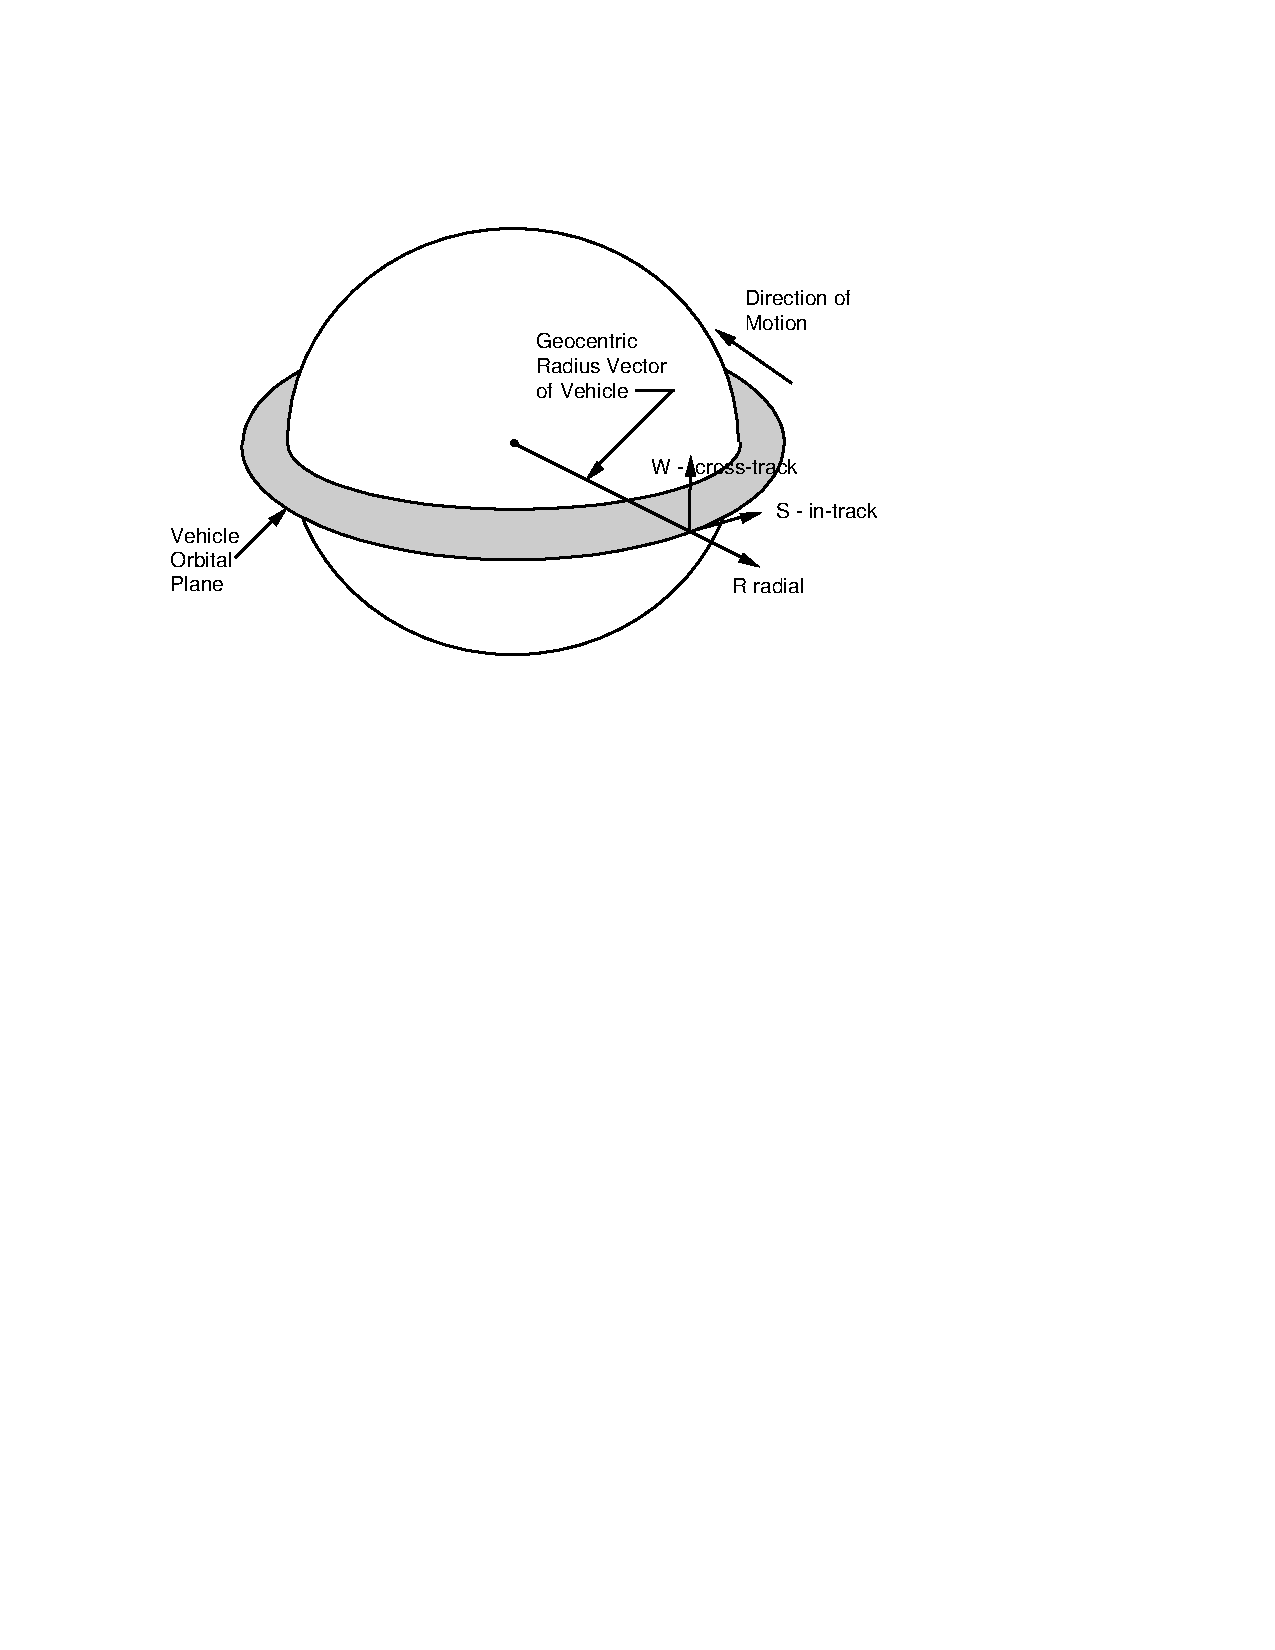
\includegraphics [width=7in]{figs/rsw.png}
\caption{RSW Coordinate System .}
\label{fig:7a}
\end{figure}
%\clearpage
%\pagebreak

\chapter{Benchmarks}\label{ap:bench}
The Integrated testing precision measured orbit fit data are located in directory:
\begin{verbatim}
/verif/Integrated_Validation/Benchmarks
the directories are:
 ROSETTA_benchmark/
 DAWN_benchmark/
 Clementine_benchmark/

 (NASA Internal Release)
 TDRS_benchmark/
 LAGEOS_benchmark/
 ISS_benchmark/
 ENVISAT_benchmark/
 CHAMP_benchmark/
 GRACE_benchmark/
\end{verbatim}
